% !Mode:: "TeX:UTF-8:Main"
\DocumentMetadata{
 lang=en,
 pdfversion=2.0,
 pdfstandard=ua-2,
 pdfstandard=a-4,
 testphase=
   {
    phase-III, %lists,footnotes,sectioning,
               %toc,marginpar,bibliography,floats,
               %graphics ...
    math,  
    table, %tabular, tabularx, longtable
    title  %maketitle
   },
 uncompress  
 }

\documentclass[12pt,a4paper]{article}
\usepackage[english]{babel}
\usepackage{microtype}
\usepackage{unicode-math}
\usepackage{graphicx}
\usepackage[autostyle]{csquotes}
\usepackage[colorlinks]{hyperref}
\hypersetup{pdftitle=The PDF Association’s work to advance accessibility,
pdfauthor=PDF Association staff}
\tagpdfsetup{role/map-tags=pdf}
\directlua{luaotfload.add_fallback
   ("emojifallback",
    {
      "Segoe UI Emoji:mode=node;"
    }
   )}

\setcounter{secnumdepth}{-1}   
\setmainfont{Arial}[RawFeature={fallback=emojifallback}]
\title{The PDF Association’s work to advance accessibility}
\author{PDF Association staff}
\begin{document}
\AddToHook{cmd/@title/before}[title]{%
\makebox[0pt][l]{\hspace*{-3cm}\raisebox{1cm}[0pt][0pt]{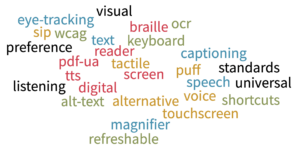
\includegraphics[scale=0.8,alt=A word-cloud of terms related to assistive technology.]{assistive-tech-word-cloud-300x150.png}}}}

\AddToHook{cmd/@author/after}{\makebox[0pt][l]{\hspace{1cm}\raisebox{4cm}[0pt][0pt]{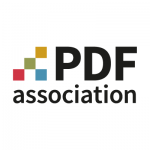
\includegraphics[alt=PDF Association staff]{PDF-Association-Logo-sq-150x150.png}}}}

\maketitle



\begin{abstract}
This article surveys the PDF Association's focus on accessibility, from
advancing accessible PDF to promoting accessibility in ISO standards
documents, and ensuring broad access and opportunity for all within its
own operations.

Founded in 2006 as the ``PDF/A Competence Center'', since 2010 the
organization has grown to encompass the PDF format as a whole. Today,
the PDF Association provides a vendor-neutral meeting-place for PDF
technology stakeholders while working to increase awareness and adoption
of ISO-standardized PDF technology, including for accessibility.
\end{abstract}

\section{ISO 14289-1 (PDF/UA-1), the ISO standard for accessible
PDF}\label{iso-14289-1-pdfua-1-the-iso-standard-for-accessible-pdf}

In 2012, after eight years of development led by PDF Association
members, ISO published
\href{https://pdfa.org/resource/iso-14289-pdfua/}{ISO 14289-1}, better
known as PDF/UA (Universal Accessibility), to define requirements for
the use of PDF's Tagged PDF feature as defined for PDF 1.7 (2008).
PDF/UA-1 was published in the early stages of the development of PDF
2.0, which began in 2009, and the lessons gained in creating PDF/UA-1
were put to use in the redevelopment of Tagged PDF in PDF 2.0.

The PDF Association caused PDF/UA-1 to be the first ISO standard
worldwide, on any subject, to itself meet standards for accessibility.
As a tagged and validated PDF file, ISO 14289-1 thus conformed, not only
with WCAG 2.0, but also with itself. 🙂

\section{Support for NVDA}\label{support-for-nvda}

Also in 2012, the PDF Association celebrated the publication of PDF/UA
by
\href{https://pdfa.org/nvda-goes-pdfua-the-pdf-association-steps-up-to-fund-development-of-the-worlds-first-pdfua-conforming-screen-reader/}{supporting
development of NVDA}, the free and open source screen reader.

\section{Best practice, test-suites and
more}\label{best-practice-test-suites-and-more}

Since the publication of PDF/UA-1 the
\href{https://pdfa.org/community/pdf-ua-technical-working-group/}{PDF/UA
TWG} and
\href{https://pdfa.org/community/pdf-accessibility-liaison-working-group/}{PDF
Accessibility LWG} have developed a variety of resources to assist
developers, end users and other stakeholders interested in driving
accessibility in PDF content. The results of these efforts include:
\begin{itemize}
\item
  \href{https://pdfa.org/resource/the-matterhorn-protocol/}{The
  Matterhorn Protocol}, now at version 1.1, is a set of tests covering
  all of PDF/UA-1's requirements.
\item
  \href{https://pdfa.org/resource/tagged-pdf-best-practice-guide-syntax/}{The
  Tagged PDF Best Practice Guide: Syntax}, provides advice beyond the
  technical requirements defined in PDF/UA.
\item
  \href{https://pdfa.org/resource/pdfua-reference-suite/}{The PDF/UA
  Reference Suite}, a set of ``real-world'' PDF files usable as a
  demonstration of how PDF files should be tagged.
\item
  \href{https://pdfa.org/resource/iso-ts-32005-hierarchical-inclusion-rules/}{Hierarchical
  inclusion rules for PDF 1.7 and PDF 2.0 structure elements} used by
  \href{https://pdfa.org/resource/iso-32005/}{ISO 32005}.
\item
  The
  \href{https://pdfa.org/glossary-of-accessibility-terminology-in-pdf/}{glossary
  of accessibility terminology in PDF}
\end{itemize}

\section{Tagged PDF redefined in ISO 32000-2 (PDF
2.0)}\label{tagged-pdf-redefined-in-iso-32000-2-pdf-2.0}

Led by the then-chairman of the PDF Association, callas software's
\href{https://pdfa.org/people/olaf-drummer/}{Olaf Drümmer}, one of PDF
2.0's most significant upgrades was the re-development of the section
defining Tagged PDF, setting the stage for PDF/UA-2.

\section{Using Tagged PDF in PDF 2.0}\label{using-tagged-pdf-in-pdf-2.0}

PDF accessibility is one of several use-cases for ``reuse'' of tagged
PDF. Other use-cases include expression as HTML, copy and paste
functionality, content extraction for use by search engines, and more.

Following publication of the 2nd edition of PDF/UA-1 in 2014, the PDF
Association's
\href{https://pdfa.org/community/pdf-ua-technical-working-group/}{PDF/UA
Technical Working Group}, later joined by the
\href{https://pdfa.org/community/pdf-reuse-twg/}{PDF Reuse TWG}, began
to develop a new specification for tagged PDF based on PDF 2.0.

Intended for publication by the PDF Association, \enquote{Using Tagged PDF in
PDF 2.0} was developed in full alignment with ISO TC 171 SC 2 WG 9, the
working group developing ISO 14289-2, to ensure its compatibility with
the forthcoming ISO standard for accessible PDF 2.0 files.

\section{ISO 14289-2 (PDF/UA-2)}\label{iso-14289-2-pdfua-2}

As mentioned above, the text of PDF/UA-2 (to be published in Q1 of 2024)
was developed by PDF Association working-groups working in coordination
with ISO's TC 171 SC 2 WG 9. Comments from the ISO committee members
were fed back into the PDF Association\textquotesingle s development
process to ensure 100\% alignment between the new ISO standard and the
PDF Association's specification for \hyperref[using-tagged-pdf-in-pdf-2.0]{Using
Tagged PDF in PDF 2.0}.

Building on PDF 2.0, PDF/UA-2 is a dramatic improvement on PDF/UA-1. For
the first time it includes comprehensive provisions for annotations and
structure element attributes, both of which are mostly absent in
PDF/UA-1. PDF/UA-2 also leverages PDF 2.0 in many other ways, from the
new Namespaces feature that allows for integration of PDF 1.7 and PDF
2.0 structure elements in the same document to MathML, the new Artifact
structure element type, and much more.

\section{Encouraging accessible ISO
standards}\label{encouraging-accessible-iso-standards}

Since 2014 the PDF Associations's PDF/UA Technical Working Group has
operated in close coordination with the ISO working group responsible
for PDF/UA, TC 171 SC 2 WG 9. Starting in 2021, members of these groups
came together to conduct an assessment of ISO's products and procedures
from the accessibility perspective. This work culminated in 2022 with
delivery to ISO of a report by the TC 171 SC 2 Chair Advisory Group
(CAG) identifying areas of concern and making recommendations for
enhancements. The PDF Association continues working actively with ISO to
identify and mitigate accessibility issues with ISO's document
production and committee workflows.

\section{Working Groups with an accessibility
focus}\label{working-groups-with-an-accessibility-focus}

As of early 2024 the PDF Association operates 20 active Working Groups.
Of these, 4 are directly engaged in advancing accessibility in PDF
technology while 2 other groups are dedicated to subjects that track
closely with accessibility.

\subsection{PDF Association WGs dedicated to
accessibility}\label{pdf-association-wgs-dedicated-to-accessibility}

\href{https://pdfa.org/community/pdf-ua-technical-working-group/}{PDF/UA
TWG} Together with the PDF Reuse TWG, this WG led development of the
specification for Using Tagged PDF in PDF 2.0, much of which will also
be published as ISO 14289-2 (PDF/UA-2).

\href{https://pdfa.org/community/pdf-accessibility-liaison-working-group/}{PDF
Accessibility LWG} This WG develops techniques for accessible PDF, with
its first set of ``fundamental'' techniques slated for publication in Q1
2024. In October 2023 the working group published an
\href{https://pdfa.org/pdf-techniques-for-accessibility-a-new-model/}{example}
of what is to come.

\href{https://pdfa.org/community/pdf-ua-processor-lwg/}{PDF/UA Processor
LWG} This WG focuses on recommendations and requirements for software
engaged in processing PDF/UA files. As of 2024 the group is focused on
examining accessibility API role mappings for HTML elements and WAI-ARIA
/ DPub attributes with the objective of mapping these features to their
functional equivalents in PDF. Check out a recent
\href{https://pdfa.org/bridging-pdf-and-web-accessibility/}{article}
about their progress.

\href{https://pdfa.org/community/latex-project-lwg/}{LaTeX Project LWG}
The \href{https://www.latex-project.org/}{LaTeX Project} is working to
enhance the LaTeX typesetting system used by academic and technical
authors worldwide to deliver complete support for the creation of
structured document formats, in particular, Tagged PDF and PDF/UA. This
LWG provides a workspace for LaTeX developers andPDF experts to share
their expertise to advance both LaTeX and Tagged PDF

\subsection{PDF Association WGs related to
accessibility}\label{pdf-association-wgs-related-to-accessibility}

\href{https://pdfa.org/community/pdf-reuse-twg/}{PDF Reuse TWG} In
addition to its collaboration with the PDF/UA TWG on the development of
Using Tagged PDF in PDF 2.0 and PDF/UA-2, this WG focuses on general
reuse of Tagged PDF to deliver advanced support for conversion to HTML,
copy and paste applications and other instances of content reuse.

\href{https://pdfa.org/community/deriving-html-from-pdf-twg/}{Deriving
HTML from PDF TWG} Author of the usage specification
``\href{https://pdfa.org/resource/deriving-html-from-pdf/}{Deriving HTML
from PDF}'' published in 2019, this working group focuses on leveraging
Tagged PDF for this common content reuse case.

\section{An ongoing commitment to
accessibility}\label{an-ongoing-commitment-to-accessibility}

PDF's core value proposition implies extreme flexibility in the
representation of content. Accordingly, although accessible PDF has been
possible for a long time, achieving it still offers challenges,
depending largely on document complexity. Accordingly, the PDF
Association will remain committed to developing resources that help all
stakeholders, software developers, institutions and end users alike, to
develop software to support accessible PDF, set policies for publication
and acquisition, and author PDF files that meet accessibility standards.
\end{document} 
